\documentclass{emulateapj}
\submitted{{\it Submitted for publication in ApJ}}
\usepackage{multirow,color,wrapfig,ulem}
\usepackage {graphicx}
%\bibliographystyle{apj}
\usepackage{graphics}
\usepackage[dvips]{epsfig}

\newcommand{\kms}{\,km~s$^{-1}$}
\def\squig{\sim\!\!}
\newcommand{\LCDM}{$\Lambda$CDM~}
\newcommand{\beq}{\begin{eqnarray}}
\newcommand{\eeq}{\end{eqnarray}}
\newcommand{\zz}{$z\sim 3$}
\newcommand{\avg}[1]{\langle{#1}\rangle}
\newcommand{\ly}{{\ifmmode{{\rm Ly}\alpha}\else{Ly$\alpha$}\fi}}
\newcommand{\hMpc}{{\ifmmode{h^{-1}{\rm Mpc}}\else{$h^{-1}$Mpc }\fi}}
\newcommand{\hGpc}{{\ifmmode{h^{-1}{\rm Gpc}}\else{$h^{-1}$Gpc }\fi}}
\newcommand{\hmpc}{{\ifmmode{h^{-1}{\rm Mpc}}\else{$h^{-1}$Mpc }\fi}}
\newcommand{\hkpc}{{\ifmmode{h^{-1}{\rm kpc}}\else{$h^{-1}$kpc }\fi}}
\newcommand{\hMsun}{{\ifmmode{h^{-1}{\rm {M_{\odot}}}}\else{$h^{-1}{\rm{M_{\odot}}}$}\fi}}
\newcommand{\hmsun}{{\ifmmode{h^{-1}{\rm {M_{\odot}}}}\else{$h^{-1}{\rm{M_{\odot}}}$}\fi}}
\newcommand{\Msun}{{\ifmmode{{\rm {M_{\odot}}}}\else{${\rm{M_{\odot}}}$}\fi}}
\newcommand{\msun}{{\ifmmode{{\rm {M_{\odot}}}}\else{${\rm{M_{\odot}}}$}\fi}}
\newcommand{\lya}{{Lyman$\alpha$~}}
\newcommand{\clara}{{\texttt{CLARA}}~}
\newcommand{\rand}{{\ifmmode{{\mathcal{R}}}\else{${\mathcal{R}}$ }\fi}}
\newcommand{\Lsun}{\mbox{\,$L_{\odot}$}}
\newcommand{\like}{\mathscr{L}}
\newcommand{\bftheta}{\mathbf{\Theta}}
\newcommand{\degree}{\ensuremath{^\circ}}
\def\spose#1{\hbox to 0pt{#1\hss}}
\def\simlt{\mathrel{\spose{\lower 3pt\hbox{$\mathchar"218$}}
     \raise 2.0pt\hbox{$\mathchar"13C$}}}
\def\simgt{\mathrel{\spose{\lower 3pt\hbox{$\mathchar"218$}}
     \raise 2.0pt\hbox{$\mathchar"13E$}}}
\font\smcap=cmcsc10
\newcommand{\YH}[1]{\textcolor{blue}{\bf YH: #1}}
\newcommand{\NEW}[1]{\textcolor{blue}{ #1}}
\newcommand{\SOUT}[1]{\textcolor{red}{\sout{ #1}}}



\shorttitle{Local Group Kinematics}
\shortauthors{Forero-Romero et al.}

\begin{document}
\title{The kinematics of the Local Group in a cosmological context}
\author{
J. E.\ Forero-Romero\altaffilmark{1},
G. Yepes\altaffilmark{2},
S. Gottl\"ober\altaffilmark{3}
}

\altaffiltext{1}{Departamento de F\'{i}sica, Universidad de los Andes, Cra. 1 No. 18A-10, Edificio Ip, Bogot\'a, Colombia, \email{je.forero@uniandes.edu.co}}
\altaffiltext{2}{Grupo de Astrof\'{\i}sica, Departamento de F\'{\i}sica Te\'orica, Universidad Aut\'onoma de Madrid,
Cantoblanco E-280049, Spain}
\altaffiltext{3}{Leibniz-Institut f\"ur Astrophysik, Potsdam, An der Sternwarte 16, 14482 Potsdam, Germany}
\date{\today}

\begin{abstract}
Multiwaveleght observations of high redshift Lyman Break Galaxies
  (LBGs) can be used to estimate the stellar mass build up at
  different cosmic epochs. Recent observational campaigns have
  extended these measurements out to $z=7$, while theoretical studies 
  show a partial success trying to account for the observational
  results at these high redshifts.
  In this paper we investigate the build up of stellar mass in Lyman Break
  Galaxies between redshifts $5\lesssim z   \lesssim 7$  with a model
  that has shown to successfully reproduce various properties   of
  LBGs and Lyman $\alpha$ emitters.  The model is
  based on the {\em MareNostrum  High-z Universe}, a large SPH
  cosmological hydrodynamical simulation. We show that the results for
  ($i$) the stellar mass as a function of observed
  UV-Luminosity, ($ii$) the integrated cosmological stellar mass   density
  (SMD) and ($iii$) the specific star formation rate (sSFR) are in good
  agreement with the results derived from observations  for bright
  galaxies with M$_{\rm UV}<-20$.  However, when taking into account
  galaxies with a fainter luminosity cut, M$_{\rm UV}<-18$, the
  results from the simulations differ systematically by a factor of two from the  observational   constraints. The deviation is such that in simulations the SMD presents a faster  redshift evolution and the sSFR is higher compared with the observations.  We also find that the extinction model that mediates the comparison between observations and simulations can have a large impact in the interpretation of these results. If the observational trends for faint high redshift galaxies are confirmed, our results hint towards the   necessity to
  improve the modeling of star formation in dwarf galaxies. 
\end{abstract}

\begin{keywords}
{galaxies: formation - galaxies: high-redshift -- methods: N-body simulations}
\end{keywords}


\section{Introduction}



The detection and detailed observational study of high redshift galaxies has
experienced a great progress during the last five years. One of the key
questions that has started to be addressed quantitatively is how fast
high redshift galaxy populations accumulate their stellar mass,
M$_{\rm star}$. Typically, the analysis is based on fits of the  Spectral Energy
Distributions (SEDs) to broad band colors of the Lyman Break Galaxies
(LBGs) population. Thanks to new observational data from the HST (WFC3/IR
and NICMOS) and Spitzer/IRAC tighter constraints to these quantities have been obtained in the
redshift range $4<z<8$ \citep{2009ApJ...697.1493S,2011ApJ...735L..34G}.       

The observations of LBGs' rest frame UV luminosity, M$_{\rm UV}$, together with the estimations of M$_{\rm star}$ allows to study
the correlation between M$_{\rm star}$ and M$_{\rm UV}$ and derived
quantities such as the integrated stellar mass density (SMD) and the
specific star formation rate (sSFR). However these estimations are
a by-product of direct measurements. Therefore, they depend on the specific
techniques and assumptions made to perform the SED fitting. 

In contrast, the stellar masses can be directly derived
from hydrodynamical simulations while M$_{\rm UV}$ is an indirect
estimate given the assumptions behind the dust extinction model and
the particular Spectral Synthesis Population Model (SSPM) used. Once
an extinction model is assumed in the simulations, a direct comparison
between the observed and simulated M$_{\rm   star}$-M$_{\rm UV}$ at
different redshifts is only possible
\citep{2011MNRAS.410.1703F,2012MNRAS.421.2568D}. Such juxtaposition,
on equal footing, between simulations and observations, provide a test
for the star formation model implemented in the simulation.  


In several previous papers
\citep{2010MNRAS.403L..31F,2011MNRAS.415.3666F,2012MNRAS.419..952F} we
have already modeled the dust extinction in such a way that we can
reproduce the general features for the observed LBG luminosity
functions (LFs), UV slopes, Lyman $\alpha$ Emitter (LAEs) LFs and also
the fraction of LBGs observed to have a strong Lyman $\alpha$ emission
at $z=5$, $6$ and $7$.  In this paper we focus on the comparison of
the stellar mass build up of simulated and observed galaxies.

This paper is structured as follows. In Sections \ref{sec:galfinder}
and \ref{sec:spectra} we review the main characteristics of the
numerical simulation and the model for extinction and
stellar continuum emission. Next, in \S \ref{sec:results} we present our
results to finalize with a discussion and conclusions in Section
\ref{sec:conclusions}.  




\section{Cosmological Simulation and Galaxy Finding}
\label{sec:galfinder}

The {\em MareNostrum  High-z Universe} simulation{\footnote{\tt
   http://astro.ft.uam.es/marenostrum}} follows the non-linear evolution of
structures in   baryons (gas and stars) and dark matter, starting  from $z=
60$  within a cube of $50\hMpc$ comoving on a side (for more details, see \cite{2010MNRAS.403L..31F}). The initial density field was sampled by $1024^3$ dark matter particles with a mass of $m_{\rm DM} = 8.2 \times 10^6 \hMsun $ and $1024^3$ SPH gas particles with a mass of $m_{\rm gas} = 1.4 \times 10^6 \hMsun$.
We have identified  the objects  using the \texttt{AMIGA} Halo
Finder\footnote{{\tt http://www.popia.ft.uam.es/AMIGA}} (\texttt{AHF})  which
is described in detail in \citet{Knollmann2009}.  All objects with  more than  $1000$
particles,  dark matter, gas and stars combined, have been used  in our analyses.

In this simulation we assumed a WMAP1 cosmology \citep{2003ApJS..148..175S}.
The favored cosmological parameters estimated from a more recent analysis of  CMB data are different from the ones used in our simulation. Therefore, we have included a correction in  the galaxy abundance based on the different number
density of dark matter halos in the cosmology used  (WMAP1 with
$\sigma_8=0.90$)  and a modern cosmology with  $\sigma_8=0.8$  which is compatible with WMAP5 \citep{2009ApJS..180..306D} and the most recent  WMAP7 data  \citep{2011ApJS..192...16L}.


\section{Spectral Modeling and UV Continuum}
\label{sec:spectra}

 The photometric properties of galaxies are calculated employing the stellar
 population synthesis model STARDUST \citep{1999A&A...350..381D} using
 the methods already described in \cite{2010MNRAS.403L..31F}. We adopt a Salpeter Initial
 Function (IMF) with lower and upper mass cut-offs of 0.1 and 120 \Msun. The Spectral Energy Distributions (SEDs)  are built from the
 AHF catalogs already described.  

The dust attenuation model parametrizes both the extinction in a
homogeneous interstellar medium (ISM) and in the molecular clouds around
young stars, following the physical model of \cite{2000ApJ...539..718C}.
The attenuation from dust in the homogeneous ISM assumes
a slab geometry, while the additional attenuation
for young stars is modeled using spherical symmetry. We refer the
reader to \cite{2010MNRAS.403L..31F} to find the exact
parametrization of the model in terms of the gas and metallicity
contents in the galaxy.

The results attained from matching the observed UV LF between redshifts
$5<z<7$ to the LFs derived from the simulation hint that all the stars younger
than $25$ Myr must be additionally extinguished for redshifts $z\sim
5,6,7$. The parameter values in the dust model are $\mu=0.03-0.01$
\citep{2010MNRAS.403L..31F}, meaning that the young stars have an
additional extinction $\mu^{-1} - 1$, ie.~$30-100$, times larger than
the extinction associated to the homogeneous ISM. Observational
constraints at $z=0$ locate $\mu$ around $1/3$ with a wide range of
scatter between $0.1$ and $0.6$ \citep{2004MNRAS.349..769K}.   

\section{Results}
\label{sec:results}

\subsection{Stellar Mass - UV luminosity scaling}


\begin{figure*}
\includegraphics[width=0.30\textwidth]{./mstar_z5.ps}\hspace{0.2cm}
\includegraphics[width=0.30\textwidth]{./mstar_z6.ps}\hspace{0.2cm}
\includegraphics[width=0.30\textwidth]{./mstar_z7.ps}
\caption{
\label{fig:mass_lum}
Stellar masses as a function of UV luminosity at redshifts $z = 5$, $6$ and
$7$. The empty  symbols represent the mean values derived from observations
\citep{2009ApJ...697.1493S,2010ApJ...716L.103L,2011ApJ...735L..34G} and the
filled hexagons the results from our simulations.  The dashed line
comes from a least square fit to the observational points at $z\sim 5$
brighter than $\mathrm{M_{\rm UV}}<-18.5$, this fit is still consistent
with the observations at $z=6$ and $7$. The continuous line at
$z=7$ represent the fit to the observational results reported by
\citet{2011MNRAS.418.2074M}.}

\end{figure*}

The scaling of the stellar mass with UV luminosity can be well described by a
function of the following form
\begin{equation}
\log_{10}\left(\frac{{\rm M_{star}}}{M_{\odot}}\right) = \alpha \times
\log_{10}\left(\frac{\mathrm{L}_{1500}}{\mathrm{erg\ s^{-1}\ Hz^{-1}}}\right)
+ \beta,
\label{eq:fit}
\end{equation}
%
where L$_{1500}$ is the UV luminosity (M$_{\rm UV}=51.63 - 2.5\times
\log_{10} ({\mathrm{L}}_{1500}[\mathrm{ergs\ s^{-1}\ Hz^{-1}}])$). In
what follows we use this parametrization to quantify our results
\citep{2011ApJ...735L..34G,2011MNRAS.418.2074M}. 


At redshift $z\sim 5$ and $z\sim 6$ the observational results come from the analysis of
deep GOODS fields, observed in the optical with the HST, in
near-infrared data from the VLT and Subaru and mid-infrared data from
Spitzer \citep{2009ApJ...697.1493S}; and the
Early Release Science (ERS) field observed with Hubble-WFC3/IR which
also counts of Spitzer/IRAC observations
\citep{2011ApJ...735L..34G}. \citet{2011ApJ...735L..34G} arrives to a result of
$\alpha =1.7\pm 0.2$ when considering the observations at $z\sim 4$
including all the points down to the faintest bin M$_{\rm  UV}\sim
-18$, this value is considered to be consistent with the data at
higher redshifts $z>4$. In both cases, the derivation of the
physical properties are done by fitting stellar synthesis models to
the observed SEDs assuming a Salpeter IMF.  Recently
\citep{2011MNRAS.418.2074M} reconsidered the data in the three deep
fields HUDF, HUDF09-2 and ERS to build a robust sample of $70$
LBGs in the redshift range $6.0<z<8.7$. From this
reanalysis they obtain the parameters $\alpha=2.14\pm0.60$ and
$\beta=-37.05\pm 4.52$ for a Chabrier IMF. We convert their results to a
Salpeter IMF by multiplying the masses by a factor of 1.8. A summary of these observations is presented in Figure \ref{fig:mass_lum}


We use the mean values of the binned observational results at $z\sim
5$ for the galaxies brighter than M$_{\rm UV}<-19.5$
\citep{2009ApJ...697.1493S,2011ApJ...735L..34G} to
make a least squares fitting to Eq. (\ref{eq:fit}). The reason
to pick this brightness cut is to dismiss a clear outlier at $z\sim 5$
in the faintest bin presented by \citet{2011ApJ...735L..34G}. From the
fit we obtain $\alpha=1.30\pm 0.08$, presented as a dashed line in  Figure
\ref{fig:mass_lum}. 

In the simulation we have calculated the stellar masses directly from the
stellar particles. The UV magnitudes include the extinction values
that were used to reproduce the LBG LF at redshifts $z=5$, $6$ and
$7$. The main results of the paper are summarized in
Fig. \ref{fig:mass_lum}. First of all, in the three studied redshifts
the values are consistent within the $1$-$\sigma$ scatter with the
observational results. However, for galaxies fainter than $M_{\rm
  UV}>-20$ at redshifts $z=5$ and $6$ the simulated data start to
deviate from the observations. At a given luminosity the
stellar mass seems to be $\sim 0.3$ dex higher than the values derived from
observations. The case at $z=7$ seems to go in the opposite
direction: the stellar masses from the simulation seem to be
lower (but sill consistent within 1$\sigma$) than the observational
estimates. Nevertheless a 0.3dex effect can be easily accounted for by different star formation histories assumed in the SED fitting procedure or other modeling choices such as the IMF or extinction law. The effect of other possible systematics in these observations has still to be considered and precisely quantified.

The mean values from the simulation can be reproduced with logarithmic slopes
$\alpha=1.18\pm0.01$, $1.26\pm0.02$ and $1.67\pm0.14$, together with intercepts $\beta=-24.61\pm 0.19$, $-26.74\pm 0.34$ and $-38.74\pm 3.87$ at redshifts $z\sim 5$, $6$ and $7$ respectively. In this fit, only the simulated galaxies brighter than
M$_{\rm UV}<-18.5$ were taken into account, which roughly correspond to
the limit of what we consider resolved objects in the
simulation. However, changing the magnitude cut down to M$_{\rm
  UV}<-18.0$ does not change significantly the results. 



\subsection{Stellar Mass Density} 

\begin{figure}
\begin{center}
\includegraphics[width=0.35\textwidth]{./mstar_dens_z.ps}
\end{center}
\caption{Stellar Mass Density (SMD) as a function of redshift for sources
  brighter than $\mathrm{M_{UV}}=-18$ (squares) and $\mathrm{M_{AB}}=-20.0$
  (triangles).  Filled symbols correspond to the results from the
  simulation. The open triangles represent the results of
  \citet{2009ApJ...697.1493S} integrating for sources brighter than
  $\mathrm{M_{UV}}=-20$, open squares refer   to the results of
  \citet{2011ApJ...735L..34G} derived from sources brighter   than
  $\mathrm{M_{UV}}=-18$. \label{fig:SMD}
}
\end{figure}


\begin{figure*}
\begin{center}
\includegraphics[width=0.35\textwidth]{./ssfr_no_ext_mstar_z.ps}\hspace{0.5cm}
\includegraphics[width=0.35\textwidth]{./ssfr_ext_mstar_z.ps}
\end{center}
\caption{The sSFR  as a function of stellar
  mass at redshifts $z=5$,$6$,$7$. In the left panel the SFR is
  estimated from the mass in star particles formed
  during the last $200$Myr. In the right panel the SFR is calculated from the
  M$_{\rm UV}$ including the effects of extinction. The
  points corresponding to $z=6$ and $z=5$ have been displaced by
  $0.025$ and $0.050$ dex respectively for clarity. The line
  approximates the loci for the median values measured at $z=6$
  \citep{2009ApJ...697.1493S} as presented in \citet{2011MNRAS.410L..42K}. 
}
\label{fig:sSFR}
\end{figure*}

In Figure \ref{fig:SMD} we show the SMD build up between redshifts
$5<z<7$. We present the SMD corresponding to different cuts M$_{{\rm UV}}$ i.e. M$_{{\rm UV}}<-20$ and M$_{\rm UV}<-18$.  For the first cut (at redshifts $z=5$, $6$, $7$) we obtain values of $\log_{10}($SMD$/\Msun$ Mpc$^{-3})$ of $6.72$, $6.05$ and $5.19$ respectively. For the cut to fainter magnitudes we get $\log_{10}$SMD$/\Msun$ Mpc$^{-3}$ of $7.25$, $6.67$ and $6.15$ at the same redshifts.

The integrated stellar mass
in the magnitude cut M$_{\rm UV}<-20$ is directly comparable to the  estimation
performed by \citet{2009ApJ...697.1493S} based on observational data at
redshifts $z\sim 5$ and $z\sim 6$. The difference between the predictions
of our simulations and the observations are less than 0.3dex. However
the trend shown by the two points at these redshifts indicate that the
stellar mass build up in the simulation is steeper than the observed one.

The steep mass growth is more evident when we include the stellar masses for
galaxies in the fainter cut M$_{\rm UV}<-18$ and compare against the observational
results by \citep{2011ApJ...735L..34G}. In their case, they extrapolate the $M/L$
ratio down to magnitudes M$_{\rm UV}=-18$, a limit below a factor
of $\sim 2$ in mass with respect the fiducial resolution for a galaxy
in the simulation. All the marked differences that were reported in
the previous section in the M$_{\rm   star}$-M$_{\rm UV}$ plane are
now translated into the SMD. At $z=5$ the normalization of the M$_{\rm
  star}$-M$_{\rm UV}$ was larger in the simulation than in the
observations, as a result the SMD value follows the same trend. At
$z=6$ and $z=7$ the M$_{\rm star}$-M$_{\rm UV}$  presents
steeper slope in observations than simulations, which is translated
into larger values of SMD by 0.2dex and 0.4dex at $z=6$ and $z=7$, 
respectively.  


\subsection{Specific Star Formation Rate}


Equivalently, the comparison between the simulation and the
observations can also be presented in terms of the specific star formation
rate, defined as sSFR$=$SFR/M$_{\rm star}$, as a function of stellar
mass. This is a less transparent procedure because of the large uncertainties in performing corrections by dust on the observed UV magnitudes.

In observations, the extinction model used to derive the stellar ages and masses is different from the model we implement \citep{2009ApJ...697.1493S,2011ApJ...735L..34G}. Ideally, a fair comparison between simulations and observations should proceed first through a SED fitting procedure to the observational data that includes the same extinction model we use, as it is the case of lower redshift work by \cite{2008MNRAS.388.1595D}.

This formal discrepancy notwithstanding, our simulation is consistent with the observed UV slopes, only the inferred amount of extinction is different. Because in observations the extinction is claimed to be negligible (justifying the use of a Madau conversion factor to calculate the SFR from the observed magnitudes) this forces us to use the \citet{1998ApJ...498..106M}  conversion formula on the extinguished magnitudes if we wish to compare our sSFR results against observations. One must keep in mind that this is technically inconsistent from the point of view of our simulation.


As a first step we verify in the simulation that the UV magnitudes uncorrected by extinction correspond to the star formation rates calculated with the widely used conversion formula in \citet{1998ApJ...498..106M}. We find that the conversion factor $c_{\rm SFR}$ between the intrinsic UV luminosity L$_{\rm UV}$ (in units of erg s$^{-1}$ Hz$^{-1}$) and the SFR (in units of \Msun yr$^{-1}$) estimated on
timescales of $\sim 0.1$ Gyr follows a relationship of the form 
L$_{\rm UV}$=$c_{\rm SFR}$ $\times$ SFR, with $c_{\rm SFR} = 1.0\times
10^{28}$ \Msun yr$^{-1}$ erg s$^{-1}$ Hz$^1$, with a 1$-\sigma$ scatter of $35\%$ between the redshifts $5<z<7$, consistent with other similar SPH simulations
\citep{2011MNRAS.410.1703F} and \citet{1998ApJ...498..106M}. 




In Figure \ref{fig:sSFR} we summarize our results. The left panel
shows the results for the sSFR from the values derived directly from
the intrinsic M$_{\rm UV}$ luminosities without any correction for
extinction. By the direct proportionality between luminosity and star formation in the simulation, this is equivalent to sampling the SFR directly from the stellar particles in the simulation. In this case the sSFR is roughly the same independent from the stellar mass of the galaxies, there is also a clear, albeit small, increase of the sSFR with redshift at all stellar
masses. This behaviour has been already noticed in semi-analytic
models \citep{2011MNRAS.417.2737W} and estimations from basic
theoretical considerations that use analytical approximations
\citep{2010ApJ...718.1001B} or semi-analytic implementations
\citep{2011MNRAS.410L..42K} that describe the gas accretion, star
formation and stellar feedback processes. 


The right panel in Figure \ref{fig:sSFR} corresponds to the values of
the SFR estimated from the attenuated values of M$_{\rm UV}$.  This corresponds to the observational assumption that the observed magnitudes are not considerably affected by extinction. This case presents a larger scatter in the values of the sSFR, lessening the
apparent redshift evolution. Furthermore, this behaviour matches, within the
intrinsic scatter of the simulated points, both the observed values
for stellar masses $\sim 10^{10}$\Msun\ at $z=6$ and the weak redshift
evolution.  The very different trends in the two panels of Figure \ref{fig:sSFR} highlight the importance of extinction corrections in shaping the sSFR. 

Nevertheless, in both estimates, the sSFR flattens at the low mass end which
is in contradiction to the observed trend at redshift z= 6.
\citep{2009ApJ...697.1493S}. As expected from the results shown in
the previous two subsections the sSFR form massive galaxies in
simulations are in agreement with observations if the dust attenuated
M$_{\rm UV}$ values are used, while for smaller systems M$_{\rm star}$
the sSFR is  systematically lower than what is
observed. \cite{2011MNRAS.410L..42K} have interpreted this result as a
hint towards stochastic increase of the stellar formation efficiency
in low mass systems. 





\section{Discussion and Conclusion}
\label{sec:conclusions}

In this paper we have presented results for the redshift evolution of
the correlation between stellar mass and UV luminosity, the integrated stellar mass
density and the specific star formation rate in Lyman Break Galaxies
at redshifts $z=5$, $6$ and $7$. We showed in previous works that the
simulated galaxies together with the dust extinction model used,
successfully reproduce the UV luminosity function, UV continuum slopes, Lyman $\alpha$
luminosity function and the fraction of LBGs with strong Lyman $\alpha$ emission \citep{2010MNRAS.403L..31F,2011MNRAS.415.3666F,2012MNRAS.419..952F}. 


We summarize here the conclusions we derive from the present analysis.

\begin{itemize}
\item At all redshifts the stellar mass and UV luminosity follow a
  tight power law, in agreement with observations.
\item With a parametrization given by $\log $M$_{\rm star} = a
  $M$_{\rm UV} + b$ (see Eq. (\ref{eq:fit}) for a precise definition),
  the simulated galaxies show a mild redshift  evolution in the
  best fit values  of $a$, while the observational values are
  reported to be consistent with no evolution \citep{2011ApJ...735L..34G}. 
\item   However, the numerical results in the
  plane M$_{\rm UV}- $M$_{\rm star}$ for   galaxies  brighter than
  M$_{\rm UV}<-20$ show a good agreement with   the observational
  estimates. Therefore, the quantitative discrepancy can be attributed
  to the behaviour of galaxies with magnitudes M$_{\rm UV}>-20$.   This discrepancy is such that, at a fixed UV luminosity, the galaxies in the simulation have larger stellar masses than in observations.
\item The integrated SMD for simulated galaxies is also in good agreement with observational
  estimates within 0.3 dex at each redshift. However, the systematic evolution is somewhat faster
  than what is inferred from observations. This seems to indicate that stars
  are formed too fast in the simulation. Again, the discrepancy is
  more clear when the smaller mass objects are included in the integration.
\item The sSFR shows differs if the SFR from
  the attenuated or non-attenuated M$_{\rm UV}$ is used. This highlights the importance of carefully  considering observational and modelling biases to interpret the  trends presented by observations as it was already suggested by  \citet{2011MNRAS.414.1927S}.  As expected from
  the results in the M$_{\rm UV}$-M$_{\rm star}$ plane, the sSFR for
  massive systems is in good agreement with observations, while the
  sSFR derived without dust attenuation is at odds with the
  observational trend. 
\end{itemize}


We conclude that our bright numerical galaxies (M$_{\rm UV}<-20$)
are consistent in all respects with the observed
galaxy populations at redshifts $5<z<7$ while there seems to be a 
discrepancy in systems with halo masses below $\sim 5\times
10^{10}$\hMsun. Although the discrepancies are only by a factor of two, the  fact that the restframe UV and Lyman$\alpha$ emission also present some tension in this mass regime, we are led to believe that a refined modelling of star formation in these galaxies is needed. Still, improved observations for the faintest high-z galaxies are required to confirm the observational trends at the faint end. If confirmed, from the theoretical point of view the solution to this conflict will have to include modifications to the standard set of assumptions behind the simulation of galaxy formation at high redshifts. A promising starting point is the examination of models including the effects of H$_2$ regulated star formation \citep{2012ApJ...749...36K} as it was suggested in the toy model implemented by \cite{2011arXiv1106.0301K}.


\section*{Acknowledgments}

We acknowledge very useful conversations with Pascal Oesch and
Valentino Gonzalez that helped to shape the final version of the
paper. The simulation used in this work is part of the MareNostrum
Numerical Cosmology Project at the BSC. The data analysis has been
performed at the NIC J\"ulich, LRZ Munich and the BABEL and EREBOS
systems at the Leibniz-Institut f\"ur Astrophysik Potsdam (AIP).

JEF-R acknowledges support from the Peter and Patricia Gruber
Foundation through their Fellowship, administered by the International
Astronomical Union. 

GY acknowledges support of  MICINN  (Spain) through research grants
FPA2009-08958, AYA2009-13875-C03-02 and Consolider SyeC (CSD2009-0050).

FP acknowledges support from the MICINN Spanish grant
AYA2010-21231-C02-01 and the Campus of International Excellence
UAM+CSIC. 

We equally acknowledge funding from the projects MULTIDARK (CSD2009-00064)
and ASTROMADRID (S2009/ESP-146). 



\bibliographystyle{apj}
\bibliography{references} 





\end{document}
